\section{Thesis Statement}

% add outline page with current section highlighted.
\begin{frame}{Outline}{$ \null $}
	%\frametitle{Outline}{ Structure }
	\tableofcontents[currentsection]
	%\tableofcontents[currentsection,currentsubsection]
\end{frame}

\begin{frame}{Thesis Statement}{ $ \null $ }

\begin{block}{ $ \null $ }

\begin{figure}
	\centering
	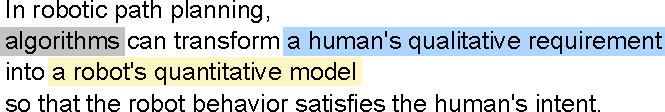
\includegraphics[width=.9\linewidth]{figure/thesis_statement1}
\end{figure}

\end{block}

\begin{figure}
	\centering
	
\includegraphics[width=.6\linewidth]{figure/thesis_statement1_fig}
\end{figure}

\end{frame}

\begin{frame}{Thesis Statement}{ $ \null $ }

\begin{block}{$ \null $}

\begin{figure}
	\centering
	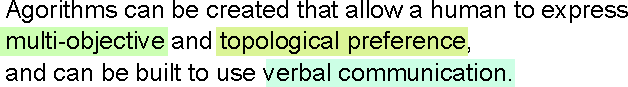
\includegraphics[width=.9\linewidth]{figure/thesis_statement2}
\end{figure}

\end{block}

\begin{figure}
	\centering
	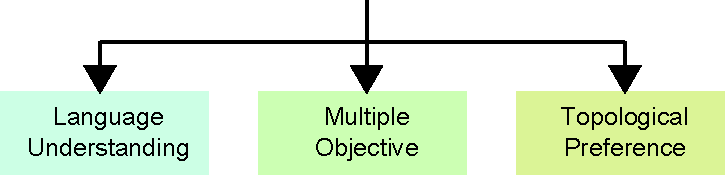
\includegraphics[width=.8\linewidth]{figure/thesis_statement2_fig}
\end{figure}

\end{frame}